\chapter{Editeur}
Pour pouvoir utiliser le logiciel de jeu existant sur d'autres morceaux, il fallait être capable de créer un document compris par le logiciel de jeu mais correspondant à d'autres musiques. Pour ce faire, nous avons créer un logiciel d'édition de morceaux, qui pouvait créer un fichier correspondant au format lu par le logiciel de jeu. Le format d'échange des données, qui est décrit plus bas, nous a donc imposé de diviser la partie editeur en deux. Chronologiquement, une première partie où l'utilisateur saisit les accords à jouer et une deuxième où il indique les moments auxquels il faut les jouer.

\section{Format d'échange}

Le format d'échange entre le logiciel de jeu et le logiciel d'édition est le même que celui qu'utilisait auparavant le logiciel de jeu.
En voici un exemple :

[INTRO]
1.914761 G
1.455219 Bm
3.149589 Em
6.328478 C
[VERSE1]
1.577916 G
1.497687 Bm
1.567347 Em

Comme nous pouvons le voir, deux voire trois éléments le compose :
\begin{itemize}
\item des annotations entre crochets
\item les notes à jouer
\item la durée de la note, qui correspond au temps entre deux notes
\end{itemize}
Pour répondre à ce format, nous avons séparés la saisi des notes et des annotations dans la première partie et la saisi des intervalles de temps dans la seconde.

\section{Saisie des notes}
\section{Saisie des temps}
Une fois la saisi des notes réalisée, l'utilisateur accède à une seconde vue pour réaliser la saisie des temps. Voici l'interface qu'aperçoit l'utilisateur :
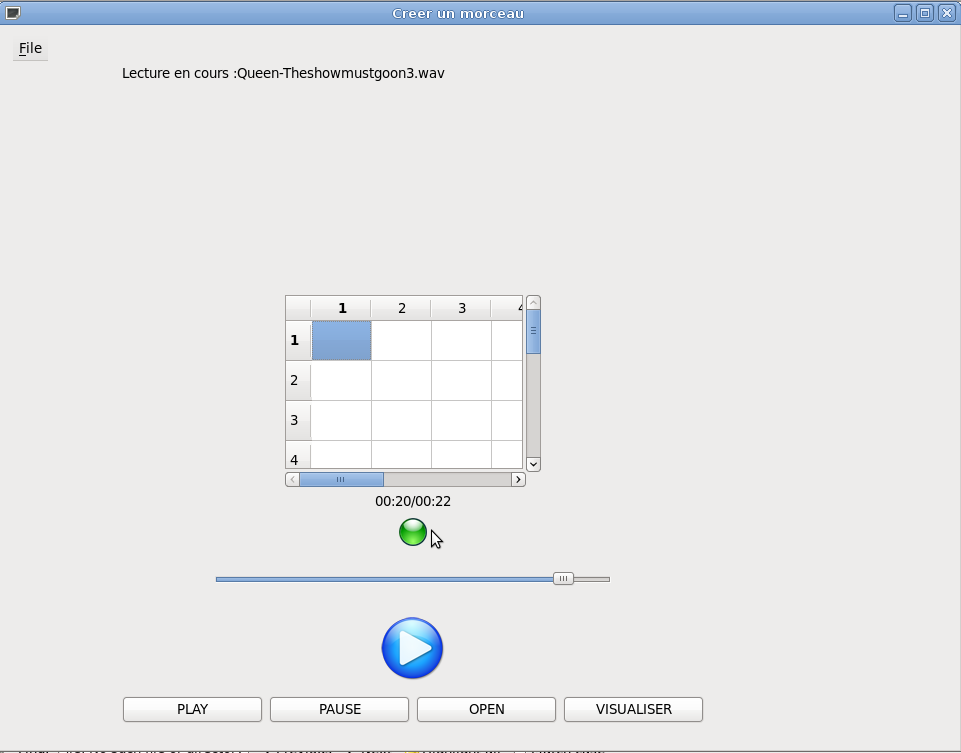
\includegraphics{editeur.png}
Nous pouvons observer, de haut en bas:
\begin{itemize}
\item nom de la piste en lecture
\item accords précédemment saisis pour lesquels il faut saisir un temps
\item la position dans la musique
\item un icone représentant l'état actuel de la musique
\item les trois boutons pour gérer la lecture de la musique ainsi que le bouton pour passer en mode visualisation
\end{itemize}
\subsection{fonctionnement}
Afin de réaliser le fichier texte correspondant à la musique que l'on veut créer, l'utilisateur commence par sélectionner le fichier wav lui correspondant. Nous avons implémenter trois facon d'ouvrir un fichier :
\begin{itemize}
\item à partir de la barre de menu file -> ouvrir une musique
\item en utilisant le raccourci clavier Ctrl + o
\item en appuyant sur le bouton play
\end{itemize}
Une fois la musique chargée, l'utilisateur dispose des fonctionnalités d'un lecteur classique, c'est-à-dire la lecture, la pause ainsi que le déplacement dans la musique en déplacant le curseur de la barre d'avancement. Il peut, bien entendu, également changer de musique en réutilisant la barre des menus ou le raccourci Ctrl + o.
Le deuxième fonctionnalité majeure est la saisi des temps où il faut jouer les accords. Pour cela, l'utilisateur doit, tout en écoutant la musique, appuyer sur la barre espace pour saisir un temps. Si l'utilisateur se trompe, il peut revenir en arrière avec le curseur de la barre d'avancement qui aura pour effet de supprimer toutes les saisies postérieures à la nouvelle postion du curseur dans la musique.
Enfin il exsite un mode de visualisation pour voir les temps saisies. Pour l'activer, il suffit de cliquer sur le bouton Visualisation, la saisie des temps sera toujours possible, mais le déplacement dans la musique ne supprime plus les temps saisies. Pour le quitter il suffit simplement de cliquer sur le bouton Stop Visualisation.
Enfin lorsque l'utilisateur est satisfait des temps et des accords saisis, il lui suffit d'exporter les données dans le format voulu en utilisant la barre des menus ou le raccourci Ctrl + e.
\subsection{implémentation}
Pour réaliser cette partie, le code a été divisé en deux. Une première classe se chargeant de la partie lecture audio et saisi des temps et une deuxième qui s'occupe de la phase de visualisation.
Lors de la création d'un nouveau morceaux, la classe createwindow se charge d'instancier un objet player, qui correspont à la première partie cité ci-dessus, et de connecter les signaux aux méthodes. Ensuite c'est l'instance du player qui se charge de créer un visualisationthread dès lors que l'utilisateur souhaite visualiser ce qu'il a déjà saisi.
Enfin pour aider l'utilisateur une barre des menus QMenuBar reste à disposition.
\subsection{correspondance avec les demandes du client}
La partie lecture audio n'ayant pas été abordé avec le client, nous nous sommes contentés des fonctionnalités de base, contrairement à la saisi des temps par la barre espace qui avait été discuté et dont nous avions trouvé accord. Un retour visuel et une visualisation possible de ce qui a été fait a été ajouté pour permettre une meilleur utilisation.
